\documentclass[UTF8, a4paper, 11pt]{ctexart}

\usepackage[margin=2.5cm]{geometry}
\usepackage{amsmath, amssymb, mathtools}
\usepackage{booktabs}
\usepackage{graphicx}
\usepackage{pgfplots}
\usepackage{siunitx}
\usepackage[hidelinks]{hyperref}

\pgfplotsset{compat=1.18}
\pgfmathdeclarefunction{arsinh}{1}{%
  \pgfmathparse{ln(#1 + sqrt((#1)*(#1) + 1))}%
}
\sisetup{per-mode=symbol}

\newcommand{\F}{F}
\newcommand{\Efield}{\mathcal{E}}
\newcommand{\dd}{\mathop{}\!\mathrm{d}}

\title{相对论匀强电场中粒子运动的\\哈密顿--雅可比理论}
\author{}
\date{\today}

\begin{document}

\maketitle

\begin{abstract}
本文以带电相对论粒子在一维匀强外电场中的运动为对象, 系统阐明哈密顿--雅可比方法将动力学问题转化为一阶偏微分方程的过程. 由相对论拉格朗日量出发, 构造正则哈密顿量及其定态哈密顿--雅可比方程, 并给出主函数的分离形式. 在此基础上, 利用正则变换常数和哈密顿方程导出满足任意初始条件的解析轨道. 文中进一步在自然单位制下比较若干横向与纵向初动量不同的初始状态, 给出 $y$--$t$, $x$--$t$ 及 $y$--$x$ 曲线. 结果表明, 纵向动量在恒力作用下线性演化, 而坐标速度受相对论色散关系约束; 横向动量守恒但横向坐标速度随总能量变化, 从而产生非抛物线型平面轨迹.
\end{abstract}

\noindent\textbf{关键词:} 哈密顿--雅可比方程; 正则变换; 相对论动力学; 匀强电场; 解析轨道

\section{引言}

哈密顿--雅可比理论在经典力学中连接了变分原理, 正则变换和可积系统理论. 与直接求解二阶运动方程不同, 该理论寻找哈密顿主函数 $S(q,P,t)$, 使其将原有相空间变量变换为常数的新正则变量. 当变换后的哈密顿量取为零时, 主函数满足哈密顿--雅可比方程, 动力学积分被归结为该方程的完备积分.

相对论粒子在匀强外场中的运动提供了一个具有物理意义的可分离模型. 相对论动能不再是动量的二次函数, 因而位置随时间的关系不同于非相对论匀加速运动. 本文讨论固定实验室参考系中的标势问题; 外场不随时间变化, 故总能量守恒. 为避免电荷符号与场方向的混淆, 以下记

\begin{equation}
  \F=e\Efield>0
\end{equation}

并取势能 $V(y)=\F y$. 于是粒子受力为 $-\F\hat y$. 所有图像均采用自然单位 $c=1$, 并以 $m=\F=1$ 的无量纲化参数作图.

\section{正则形式与哈密顿--雅可比方程}

对于具有 $n$ 个自由度的系统, 定义正则动量与哈密顿量为

\begin{equation}
  p_i=\frac{\partial L}{\partial\dot q^i}
  \qquad
  H(q,p,t)=p_i\dot q^i-L(q,\dot q,t)
\end{equation}

在勒让德变换非退化的条件下, 哈密顿正则方程为

\begin{equation}
  \dot q^i=\frac{\partial H}{\partial p_i}
  \qquad
  \dot p_i=-\frac{\partial H}{\partial q^i}
  \label{eq:hamilton}
\end{equation}

取第二类生成函数 $S(q,P,t)$, 其中 $P_i$ 是新动量. 由正则一形式的关系

\begin{equation}
  \dd S=p_i\dd q^i+Q^i\dd P_i+(K-H)\dd t
\end{equation}

可得

\begin{equation}
  p_i=\frac{\partial S}{\partial q^i}
  \qquad
  Q^i=\frac{\partial S}{\partial P_i}
  \qquad
  K=H+\frac{\partial S}{\partial t}
  \label{eq:canonical-transform}
\end{equation}

若能选择 $S$ 使新哈密顿量 $K$ 为零, 则 $P_i$ 与 $Q^i$ 均为运动常数. 式 \eqref{eq:canonical-transform} 随即给出哈密顿--雅可比方程

\begin{equation}
  \frac{\partial S}{\partial t}
  +H\left(q,\frac{\partial S}{\partial q},t\right)=0
  \label{eq:hj}
\end{equation}

当 $H$ 不显含时间时, 设 $S=W(q,P)-\varepsilon t$, 其中 $\varepsilon$ 是守恒能量, 则 \eqref{eq:hj} 化为定态方程

\begin{equation}
  H\left(q,\frac{\partial W}{\partial q}\right)=\varepsilon
  \label{eq:time-independent-hj}
\end{equation}

\section{相对论粒子的可分离解}

考虑质量为 $m$ 的粒子在 $x$--$y$ 平面内运动. 相对论拉格朗日量为

\begin{equation}
  L=-m\sqrt{1-\dot x^2-\dot y^2}-\F y
  \label{eq:lagrangian}
\end{equation}

相应的正则动量和哈密顿量为

\begin{equation}
  p_x=\frac{m\dot x}{\sqrt{1-\dot x^2-\dot y^2}}
  \qquad
  p_y=\frac{m\dot y}{\sqrt{1-\dot x^2-\dot y^2}}
\end{equation}

\begin{equation}
  H=\sqrt{m^2+p_x^2+p_y^2}+\F y
  \label{eq:relativistic-hamiltonian}
\end{equation}

由于 $x$ 为循环坐标, 取分离常数 $a=p_x$, 并写作 $W(x,y)=ax+W_y(y)$. 由 \eqref{eq:time-independent-hj} 得

\begin{equation}
  \left(\frac{\dd W_y}{\dd y}\right)^2
  =(\varepsilon-\F y)^2-m^2-a^2
  \label{eq:separated}
\end{equation}

在固定动量分支上, 令 $b=\sqrt{m^2+a^2}$ 及 $u=\varepsilon-\F y$, 则一个特征函数为

\begin{equation}
  W=ax-\frac{1}{2\F}
  \left[
    u\sqrt{u^2-b^2}
    -b^2\ln\left(u+\sqrt{u^2-b^2}\right)
  \right]
  \label{eq:characteristic-function}
\end{equation}

式 \eqref{eq:characteristic-function} 仅在指定根号和对数分支上成立. 不同的初始纵向动量对应不同的局部支, 但由同一守恒量描述. 相比显式使用 \eqref{eq:characteristic-function} 消去积分常数, 直接对 \eqref{eq:relativistic-hamiltonian} 应用 \eqref{eq:hamilton} 更便于写出满足初始条件的轨道.

\section{由初始条件确定的解析轨道}

令 $t=0$ 时的位置和动量为 $(x_0,y_0,p_{x0},p_{y0})$. 由 \eqref{eq:hamilton} 可知

\begin{equation}
  p_x(t)=p_{x0}
  \qquad
  p_y(t)=p_{y0}-\F t
  \label{eq:momentum-evolution}
\end{equation}

定义

\begin{equation}
  b=\sqrt{m^2+p_{x0}^2}
  \qquad
  \omega(t)=\sqrt{b^2+\left(p_{y0}-\F t\right)^2}
  \qquad
  \omega_0=\omega(0)
\end{equation}

由 $\dot y=p_y/\omega$ 和 $\dot x=p_{x0}/\omega$ 积分, 得到

\begin{align}
  y(t)
  &=y_0+\frac{\omega_0-\omega(t)}{\F}
  \label{eq:y-of-t}\\
  x(t)
  &=x_0+\frac{p_{x0}}{\F}
  \left[
    \operatorname{arsinh}\left(\frac{p_{y0}}{b}\right)
    -\operatorname{arsinh}\left(\frac{p_{y0}-\F t}{b}\right)
  \right]
  \label{eq:x-of-t}
\end{align}

由 \eqref{eq:y-of-t} 可见, $p_y=0$ 时粒子达到最大的 $y$ 坐标, 随后向负 $y$ 方向运动. 该转折时刻为 $t_\mathrm{turn}=p_{y0}/\F$, 仅当 $p_{y0}>0$ 时位于 $t>0$ 区间. 另一方面, 尽管 $p_x$ 守恒, $\dot x=p_{x0}/\omega(t)$ 一般不守恒, 因为纵向动量改变了总能量 $\omega(t)$.

\section{不同初始条件下的轨道比较}

为比较轨道族, 以下固定 $x_0=y_0=0$, $m=\F=1$, 并在 $0\le t\le 4$ 范围内绘图. 表 \ref{tab:initial-conditions} 列出四组初始动量. 第一组对应纯纵向释放, 第二组引入横向动量, 第三组具有正的初始纵向动量并出现转折点, 第四组则从初始时刻起向负 $y$ 方向运动.

\begin{table}[htbp]
  \centering
  \caption{用于绘图的无量纲初始条件}
  \label{tab:initial-conditions}
  \begin{tabular}{cccc}
    \toprule
    轨道 & $p_{x0}$ & $p_{y0}$ & 物理特征 \\
    \midrule
    A & $0$   & $0$    & 纯纵向运动 \\
    B & $0.8$ & $0$    & 无初始纵向动量的斜向运动 \\
    C & $0.8$ & $1.2$  & 先上升后转折 \\
    D & $1.4$ & $-0.6$ & 初始即向负 $y$ 方向运动 \\
    \bottomrule
  \end{tabular}
\end{table}

\begin{figure}[htbp]
  \centering
  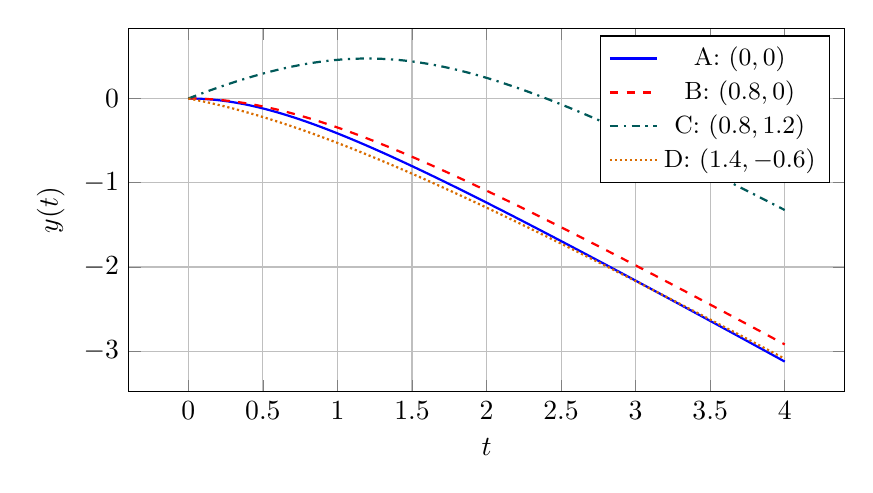
\begin{tikzpicture}
    \begin{axis}[
      width=0.88\textwidth,
      height=6.2cm,
      xlabel={$t$},
      ylabel={$y(t)$},
      grid=both,
      legend style={at={(0.98,0.98)}, anchor=north east, font=\small},
      domain=0:4,
      samples=200,
    ]
      \addplot[blue, thick] {1-sqrt(1+x^2)};
      \addlegendentry{A: $(0,0)$}
      \addplot[red, thick, dashed] {sqrt(1+0.8^2)-sqrt(1+0.8^2+x^2)};
      \addlegendentry{B: $(0.8,0)$}
      \addplot[teal!70!black, thick, dashdotted] {sqrt(1+0.8^2+1.2^2)-sqrt(1+0.8^2+(1.2-x)^2)};
      \addlegendentry{C: $(0.8,1.2)$}
      \addplot[orange!85!black, thick, densely dotted] {sqrt(1+1.4^2+0.6^2)-sqrt(1+1.4^2+(-0.6-x)^2)};
      \addlegendentry{D: $(1.4,-0.6)$}
    \end{axis}
  \end{tikzpicture}
  \caption{不同初始动量下的纵向坐标 $y(t)$. 图例中括号内依次为 $(p_{x0},p_{y0})$.}
  \label{fig:y-t}
\end{figure}

\begin{figure}[htbp]
  \centering
  \begin{tikzpicture}
    \begin{axis}[
      width=0.88\textwidth,
      height=6.2cm,
      xlabel={$t$},
      ylabel={$x(t)$},
      grid=both,
      legend style={at={(0.02,0.98)}, anchor=north west, font=\small},
      domain=0:4,
      samples=200,
    ]
      \addplot[blue, thick] {0};
      \addlegendentry{A: $(0,0)$}
      \addplot[red, thick, dashed] {0.8/sqrt(1+0.8^2)*(arsinh(0/sqrt(1+0.8^2))-arsinh((0-x)/sqrt(1+0.8^2)))};
      \addlegendentry{B: $(0.8,0)$}
      \addplot[teal!70!black, thick, dashdotted] {0.8/sqrt(1+0.8^2)*(arsinh(1.2/sqrt(1+0.8^2))-arsinh((1.2-x)/sqrt(1+0.8^2)))};
      \addlegendentry{C: $(0.8,1.2)$}
      \addplot[orange!85!black, thick, densely dotted] {1.4/sqrt(1+1.4^2)*(arsinh(-0.6/sqrt(1+1.4^2))-arsinh((-0.6-x)/sqrt(1+1.4^2)))};
      \addlegendentry{D: $(1.4,-0.6)$}
    \end{axis}
  \end{tikzpicture}
  \caption{不同初始动量下的横向坐标 $x(t)$. 纯纵向轨道 A 满足 $x(t)=0$.}
  \label{fig:x-t}
\end{figure}

\begin{figure}[htbp]
  \centering
  \begin{tikzpicture}
    \begin{axis}[
      width=0.88\textwidth,
      height=7cm,
      xlabel={$x$},
      ylabel={$y$},
      grid=both,
      legend style={at={(0.02,0.02)}, anchor=south west, font=\small},
      domain=0:4,
      samples=200,
    ]
      \addplot[blue, thick] coordinates {(0,0) (0,-3.1231)};
      \addlegendentry{A: $(0,0)$}
      \addplot[red, thick, dashed] (
        {0.8/sqrt(1+0.8^2)*(arsinh(0/sqrt(1+0.8^2))-arsinh((0-x)/sqrt(1+0.8^2)))},
        {sqrt(1+0.8^2)-sqrt(1+0.8^2+x^2)}
      );
      \addlegendentry{B: $(0.8,0)$}
      \addplot[teal!70!black, thick, dashdotted] (
        {0.8/sqrt(1+0.8^2)*(arsinh(1.2/sqrt(1+0.8^2))-arsinh((1.2-x)/sqrt(1+0.8^2)))},
        {sqrt(1+0.8^2+1.2^2)-sqrt(1+0.8^2+(1.2-x)^2)}
      );
      \addlegendentry{C: $(0.8,1.2)$}
      \addplot[orange!85!black, thick, densely dotted] (
        {1.4/sqrt(1+1.4^2)*(arsinh(-0.6/sqrt(1+1.4^2))-arsinh((-0.6-x)/sqrt(1+1.4^2)))},
        {sqrt(1+1.4^2+0.6^2)-sqrt(1+1.4^2+(-0.6-x)^2)}
      );
      \addlegendentry{D: $(1.4,-0.6)$}
    \end{axis}
  \end{tikzpicture}
  \caption{平面轨迹 $y(x)$ 的参数表示. 参数为时间 $t$, 范围为 $0\le t\le4$.}
  \label{fig:y-x}
\end{figure}

图 \ref{fig:y-t} 至图 \ref{fig:y-x} 与解析式 \eqref{eq:y-of-t}, \eqref{eq:x-of-t} 一致. 轨道 C 在 $t=1.2$ 处达到最高点; 这是其初始正纵向动量被外力完全抵消的时刻. 轨道 B 与 C 的 $p_{x0}$ 相同, 但 C 在初期具有较大的总能量, 故其初始横向坐标速度较小. 轨道 A 在 $x=0$ 上退行, 而其余三条轨道由于 $p_{x0}>0$ 向正 $x$ 方向单调推进. 曲线的非抛物线性质源于相对论关系 $\omega^2=m^2+p_x^2+p_y^2$, 而非坐标加速度为常数的假设.

\section{结论}

本文从相对论拉格朗日量建立了带电粒子在匀强电场中的哈密顿描述, 并通过哈密顿--雅可比方程给出可分离的特征函数. 以初始相空间点为参数, 得到了位置与时间的显式解析关系. 该表达式同时揭示了两项相对论效应: 纵向坐标不再具有二次时间依赖, 横向动量虽守恒但横向速度随纵向动量及总能量改变. 所给三类图像展示了这些结论对不同初始条件的具体表现, 也为进一步研究时变场, 磁场或曲时空背景中的可积相对论系统提供了基准模型.

\end{document}
